%!TEX root=report.tex

\subsection{OLS with autocorrelated residuals}
Since the OLS model with autocorrelated residuals, requires an equidistant time series a linear interpolation \todo{Confirm that it is linear}, was used to fill in the gaps in the GRACE data. 

The difference between OLS with and without autocorrelated residuals, was then examined for a multitude of different locations on the globe. In this examination the result was generally the same, $\hat{y}$ wasn't changed very much, but the $\hat{\sigma}_\epsilon^2$ quite a bit smaller.

\begin{figure}[H]
\centering
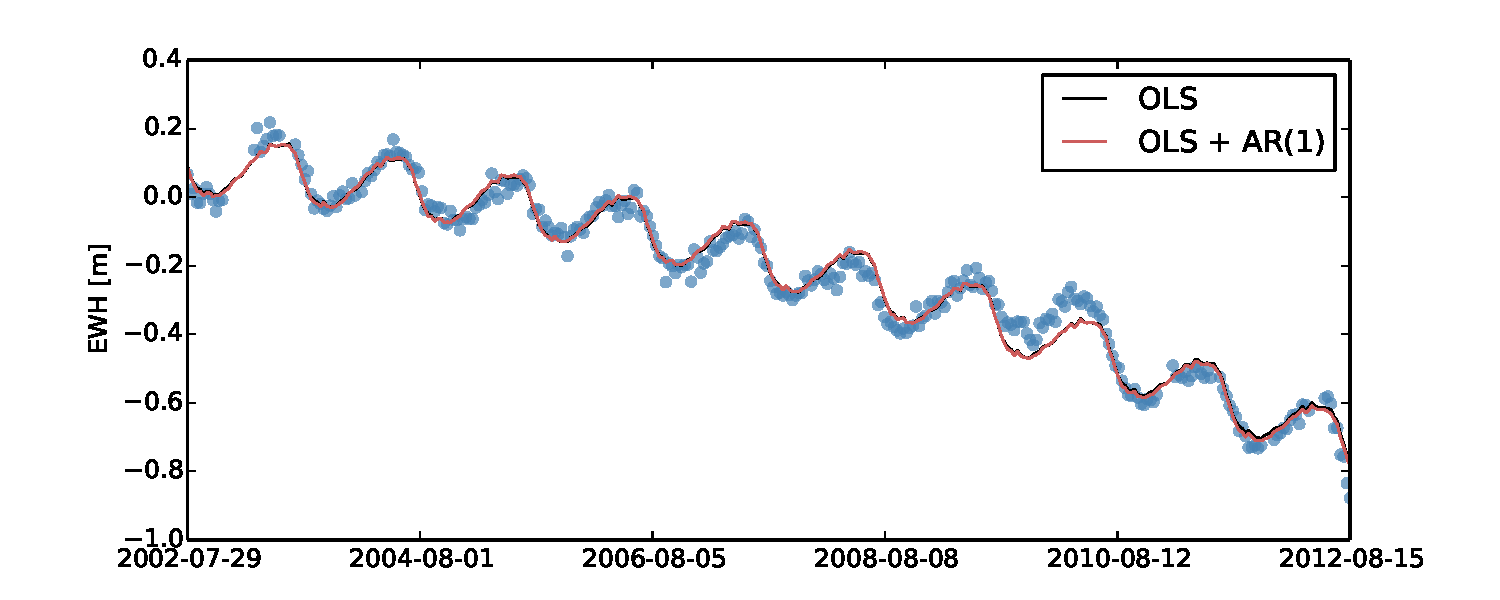
\includegraphics[width=1.0\textwidth]{figures/ar-compare}
\caption{OLS and OLS with autocorrrelated residuals. Position is 63.5 N 49.5 W, west coast of Greenland.}
\label{fig:ar-compare}
\end{figure}

\begin{table}[H]
\centering
\begin{tabular}{r | l l}
                             & OLS    & OLS+AR(1) \\ \hline
$\rho$		 & 0          & 0.773 \\
$\hat{\sigma}_\epsilon^2$ & $1.35 \cdot 10^{-3}$ & $ 5.64 \cdot 10^{-4}$ \\
MSR                   & 43.027 & 43.482 \\
Durbin-Watson & 0.477 & 2.328
\end{tabular}
\caption{Summarized difference between OLS with and without autocorrelated residuals}
\label{table:ar-compare}
\end{table}

From Figure \ref{fig:ar-compare} it is seen that the $\hat{y}$ is almost identical, which is because the $\hat{\beta}$ parameters are almost identical. One could have hoped for a better result here, but the reason for the poor fit is properly that the season length aren't the same each year and correcting for autocorrelated residuals won't do much difference here.

In Table \ref{table:ar-compare} the its seen that the MSE ($\sum_{i=1}^n (y_i - \hat{y}_i)^2$, not interpolated) is similar unchanged. The estimated variance and the Durbin-Watson test statistics is however much improved. This suggests that the OLS overestimated the noise variance of the data. The result should be that the p-value are more correct and in this case more parameters should be significantly different from zero.
